\documentclass{standalone}
\usepackage{tikz}
\usepackage{ctex,siunitx}
\setCJKmainfont{Noto Serif CJK SC}
\usepackage{tkz-euclide}
\usepackage{amsmath}
\usepackage{wasysym}
\usetikzlibrary{patterns, calc}
\usetikzlibrary {decorations.pathmorphing, decorations.pathreplacing, decorations.shapes,}
\begin{document}
\small
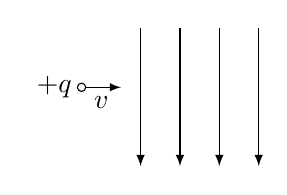
\begin{tikzpicture}[>=latex,scale=0.5]
  \foreach \x in {1,...,4}
  {
          \draw [<-](\x,0.5)--(\x,4);
  }
  \draw [->] (-.5,2.5)node [left]{$+q$}--node [below]{$v$}(0.5,2.5);
  \draw (-.5,2.5)[fill=white] circle (3pt);
\end{tikzpicture}
\end{document}